\documentclass[12pt]{article}
\usepackage{graphicx}
\usepackage{geometry}
\usepackage{titlesec}
\usepackage{fancyhdr}

% Geometry settings
\geometry{a4paper, margin=1in}

% Title formatting
\titleformat{\section}{\normalfont\Large\bfseries}{\thesection}{1em}{}

% Header and footer settings
\pagestyle{fancy}
\fancyhf{}
\fancyhead[L]{Microcontrollers and Microprocessors \\ Biomedical Signal Processing}
\fancyhead[R]{\thepage}
\fancyfoot[L]{Submitted to: Miss Sahar Batool}
\fancyfoot[R]{Date: 29/05/2024}

% Title page
\title{
    \vspace{-2cm}
    
\includegraphics[width=0.3\textwidth]{logo.png}\\ % Include your institution logo if available
    \vspace{1cm}
    \textbf{Project Report:}\\
    \textbf{ECG Signal Processing Using AD8232 and Arduino}
}
\author{
    \textbf{Team Members:} \\
    Dua Farooq \\
    Javeria Ahmed
}
\date{29/05/2024}

\begin{document}

\maketitle
\newpage

\tableofcontents
\newpage

\section{Objective}
To assemble and process ECG signals using AD8232 sensor module, Arduino, and MATLAB for real-time monitoring and variability analysis, aiming to detect normal and affected ECG signals.

\section{Introduction}
Electrocardiography (ECG) is a crucial tool in monitoring heart activity. This project involves using a microcontroller-based setup to capture and process ECG signals. The AD8232 sensor module is used to collect ECG signals, which are then processed and analyzed using Arduino and MATLAB. This approach provides real-time monitoring and analysis of cardiac health, demonstrating the capabilities of microcontrollers in biomedical signal processing.

\section{Block Diagram / Schematic}
\begin{figure}[h!]
    \centering
    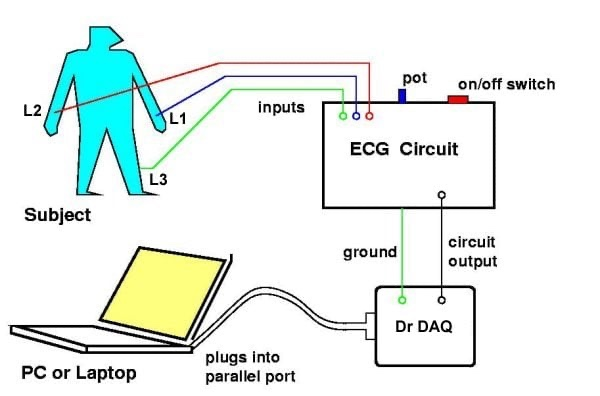
\includegraphics[width=0.8\textwidth]{schematic.jpeg}
    \caption{Block Diagram of the ECG Signal Processing Setup}
    \label{fig:block_diagram}
\end{figure}

\section{Procedure}
\subsection{Hardware Part 1/2 - Assemble Hardware}
\begin{enumerate}
    \item Connect the AD8232 module to the Arduino using jumper wires.
    \item Attach the ECG electrodes to the AD8232 module.
    \item Place the electrodes on the subject's body to capture the ECG signal.
    \item Connect the Arduino to a breadboard for power and signal routing.
\end{enumerate}

\subsection{Hardware Part 2/2 - Show Signal in IDE}
\begin{enumerate}
    \item Open the Arduino IDE and select the appropriate board and port.
    \item Upload a sketch to read the analog signal from the AD8232 module.
    \item Use the Serial Monitor to visualize the ECG signal in real-time.
\end{enumerate}

\subsection{Software Part 1/2 - Export Signal to MATLAB (Normal ECG)}
\begin{enumerate}
    \item Use the Arduino IDE to export the captured ECG data to a CSV file.
    \item Import the CSV file into MATLAB.
    \item Plot the ECG signal in MATLAB to verify normal heart activity.
\end{enumerate}

\subsection{Software Part 2/2 - Show Variability of Signal in MATLAB (Affected ECG)}
\begin{enumerate}
    \item Analyze the ECG signal in MATLAB to detect any abnormalities.
    \item Use signal processing techniques to highlight variability in the ECG signal.
    \item Compare normal and affected ECG signals to identify differences.
\end{enumerate}

\section{Results and Plots}
% \begin{figure}[h!]
%     \centering
%     \includegraphics[width=0.8\textwidth]{normal_ecg.png}
%     \caption{Normal ECG Signal Exported to MATLAB}
%     \label{fig:normal_ecg}
% \end{figure}

% \begin{figure}[h!]
%     \centering
%     \includegraphics[width=0.8\textwidth]{affected_ecg.png}
%     \caption{Affected ECG Signal Showing Variability}
%     \label{fig:affected_ecg}
% \end{figure}

\section{Discussion / Key Points}
\begin{itemize}
    \item The AD8232 module effectively captures ECG signals with good clarity.
    \item Real-time visualization in Arduino IDE helps in immediate monitoring.
    \item MATLAB provides robust tools for detailed analysis and visualization of ECG signals.
    \item Signal variability analysis can help in detecting cardiac conditions such as ischemia.
\end{itemize}

\section{Summary}
This project demonstrates the integration of microcontrollers and signal processing software to capture, visualize, and analyze ECG signals. The hardware setup using AD8232 and Arduino allows real-time monitoring, while MATLAB aids in detailed analysis, making it a powerful combination for biomedical applications.

\section{Feature Extraction: Cardiac Ischemia}
Using MATLAB, features such as QRS complex, P wave, and T wave can be extracted from the ECG signal. Abnormalities in these features can indicate cardiac ischemia. Automated feature extraction algorithms can enhance the diagnostic process.

\section{Real-Time Output}
The real-time output from the Arduino setup provides immediate feedback on heart activity. This can be crucial for continuous monitoring and early detection of cardiac issues.

\section{Materials}
\begin{itemize}
    \item Breadboard
    \item Jumper wires
    \item AD8232 module
    \item Arduino IDE
    \item MATLAB
    \item Arduino
\end{itemize}

\end{document}
